% Configuration
\documentclass[a4paper, 10pt]{article}

% Formatting
\usepackage[landscape, left=0.75cm, top=1.0cm, right=0.75cm, bottom=1.5cm, footskip=15pt]{geometry}
\setlength{\columnsep}{0.5cm}
\usepackage{flowfram}
\ffvadjustfalse
\Ncolumn{3}
\usepackage[compact]{titlesec}

% ------------------------
% Imports and commands
% ------------------------

% Language stuff
\usepackage[english]{babel}
\usepackage[utf8]{inputenc}

% Math stuff
\usepackage{amsthm}
\usepackage{amssymb}
\usepackage{amsmath}

\newtheorem*{corollary}{Cor}
\newtheorem*{lemma}{Lemma}

\theoremstyle{definition}
\newtheorem*{theorem}{Thm}
\newtheorem*{definition}{Def}
\newtheorem*{note_wrapper}{Hint}

\newtheoremstyle{named}{}{}{}{}{\bfseries}{.}{.5em}{\thmnote{#3}}
\theoremstyle{named} 
\newtheorem*{ntheorem_wrapper}{Theorem}

% Colored boxes
\usepackage{xcolor}
\usepackage{mdframed}
\mdfsetup{skipabove=-2pt,skipbelow=-2pt}

\definecolor{cwhite}{HTML}{d7dbd7}
\mdfdefinestyle{important}{
    linecolor=yellow,
    linewidth=0pt,
    innertopmargin=-6pt,
    innerbottommargin=2pt,
    innerrightmargin=2pt,
    innerleftmargin=2pt,
    leftmargin=0pt,
    rightmargin=0pt,
    outerlinewidth=0pt,
    backgroundcolor=cwhite,
}

\newenvironment{ntheorem}%
    {\begin{mdframed}[style=important]\begin{ntheorem_wrapper}}%
    {\end{ntheorem_wrapper}\end{mdframed}}

\definecolor{cgreen}{HTML}{2ecc71} 
\mdfdefinestyle{trick}{
    linecolor=yellow,
    linewidth=0pt,
    innertopmargin=-6pt,
    innerbottommargin=2pt,
    innerrightmargin=2pt,
    innerleftmargin=2pt,
    leftmargin=0pt,
    rightmargin=0pt,
    outerlinewidth=0pt,
    backgroundcolor=cgreen,
}

\newenvironment{note}%
    {\begin{mdframed}[style=trick]\begin{note_wrapper}}%
    {\end{note_wrapper}\end{mdframed}}

% Table stuff
\usepackage{tabularx} % tabularx since the width should be handled automatically
\usepackage{booktabs}

% Graph stuff
\usepackage{pgfplots}

% Miscellaneous
\usepackage{hyperref}
\hypersetup{colorlinks=true, urlcolor=blue, linkcolor=blue, citecolor=blue}

\usepackage{enumitem}
\setitemize{itemsep=0.5pt, topsep=0pt}
\setenumerate{itemsep=0.75pt}

% Custom commands
\newcommand{\R}{\mathbb{R}}
\newcommand{\Q}{\mathbb{Q}}
\newcommand{\N}{\mathbb{N}}
\newcommand{\Z}{\mathbb{Z}}
\newcommand{\C}{\mathbb{C}}
\newcommand{\BO}{\mathcal{O}}
\renewcommand{\labelenumii}{\arabic{enumi}.\arabic{enumii}}

% Metadata
\title{Analysis I Summary}
\author{Nicola Studer \\ \href{mailto:nicstuder@student.ethz.ch}{nicstuder@student.ethz.ch}}
\date{\today}


% ------------------------
% Document
% ------------------------

\begin{document}
\maketitle

\section{Real numbers, euclidean spaces}
\begin{ntheorem}[Archimedes' principle]
    If $x \in \R$ with $x > 0$ and $y \in \R$, then $\exists n \in \N \ (y \leq n \cdot x)$
\end{ntheorem}

\begin{theorem}
    \begin{enumerate}[label=(\roman*)]
        \item $|x| \geq 0 \quad \forall x \in \R$
        \item $|xy| = |x||y| \quad \forall x, y \in \R$
        \item $|x + y| \leq |x| + |y| \quad \forall x, y \in \R$
        \item $|x + y| \geq ||x| - |y|| \quad \forall x, y \in \R$
    \end{enumerate}
\end{theorem}

\begin{ntheorem}[Young's inequality]
    $\forall \epsilon > 0, \forall x, y \in \R$:
    $$2 |xy| \leq \epsilon x^2 + \frac{1}{\epsilon} y^2$$
\end{ntheorem}

\section{Sequences}
\subsection{Convergence}
$(a_n)_{n \geq 1}$ converges to $L = \lim_{n \to \infty} a_n$ \\
$\iff \forall \epsilon > 0 \ \exists N \in \N \ \forall n > N \ (|a_n - L | < \epsilon)$

\begin{definition}[Convergence]
    $(a_n)_{n \geq 1}$ converges \\
    $\iff \exists L \in \R  \ \forall \epsilon > 0 \ (\{n \in \N \ | \ |a_n - L| \geq \epsilon \})$ is finite.
\end{definition}

\begin{note}
    Let $(a_n)_{n\geq1}$, $(b_n)_{n\geq1}$ converge with limit $a$ and $b$:
    \begin{enumerate}
        \item $(a_n + b_n)_{n\geq1}$ converges with limit $a + b$
        \item $(a_n \cdot b_n)_{n\geq1}$ converges with limit $a \cdot b$.
        \item $(\frac{a_n}{b_n})_{n\geq1}$ converges with limit $\frac{a}{b}$
        \item $\exists K \geq 1 \ \forall n \geq K: a_n \leq b_n \implies a \leq b$
    \end{enumerate}
\end{note}

\subsubsection{Tips \& Tricks}
\begin{itemize}
    \item $a_n$ convergent $\implies$ $a_n$ bounded
    \item $a_n$ convergent $\iff$ $a_n$ bounded and \\ 
    $\lim\inf a_n = \lim\sup a_n$
\end{itemize}

\begin{ntheorem}[Monotone Convergence]
    $(a_n)_{n \geq 1}$ monotone increasing and upper bounded $\implies$ $\lim a_n = \sup\{a_n \ | \ n\geq 1\}$ \newline
    $(a_n)_{n \geq 1}$ monotone decreasing and lower bounded $\implies$ $\lim a_n = \inf\{a_n \ | \ n\geq 1\}$
\end{ntheorem}

\begin{lemma}[Bernoulli Inequation]
    $$(1 + x)^n \geq 1 + nx \quad \forall n \in \N, x > -1$$
\end{lemma}

\begin{definition}[Limit inferior / Limit superior]
    $$\underset{n\to\infty}{\lim\inf} \ a_n \ := \ \lim_{n\to\infty} (\inf \{a_k \ | \ k \geq n\})$$
    $$\underset{n\to\infty}{\lim\sup} \ a_n \ := \ \lim_{n\to\infty} (\sup \{a_k \ | \ k \geq n\})$$
\end{definition}

\begin{ntheorem}[Cauchy Criteria]
    $a_n$ converges iff $\forall \epsilon > 0 \ \exists N \geq 1$ s.t. $|a_n - a_m| < \epsilon$ $\forall n,m \geq N$ (cauchy sequence).
    \begin{enumerate}[label=(\roman*)]
        \item Each Cauchy sequence is bounded
        \item $(a_n)_{n \geq 1}$ conv. $\implies (a_n)_{n \geq 1}$ cauchy
        \item $(a_n)_{n \geq 1}$ cauchy $\implies (a_n)_{n \geq 1}$ conv.
    \end{enumerate}
\end{ntheorem}

\begin{ntheorem}[Bolzano-Weierstrass]
    Each bounded sequence contains a convergent sub sequence.
\end{ntheorem}

\begin{ntheorem}[Sandwich]
    If $\lim a_n = \alpha$, $\lim b_n = \alpha$, $k \in \N$ and \\
    $a_n \leq c_n \leq b_n$ $\forall n \geq k$, then $\lim c_n = \alpha$
\end{ntheorem}

\begin{ntheorem}[Cauchy-Cantor]
    Let $I_1 \supseteq I_2 \supseteq \cdots I_n \cdots$ be a sequence of proper intervals with $\mathcal{L} < + \infty$, then $\bigcap_{n\geq1} I_n \neq 0$. And if $\lim_{n \to \infty} \mathcal{L}(I_n) = 0$ then $|\bigcap_{n\geq1} I_n| = 1$
\end{ntheorem}

\begin{corollary}
    Let $(a_n)$ be bounded, then for each subsequence $(b_n)$: $\liminf a_n \leq \lim b_n \leq \limsup a_n$.

    Each subsequence $(b_n)$ of a convergent $(a_n)$ converges and $\lim b_n = \lim a_n$.
\end{corollary}

\section{Series}
\begin{definition}
    "$\sum_{k=1}^\infty a_k$" converges, if the sequence $(S_n)_{n \geq 1}$ of partial sums converges and $\sum\limits_{k=1}^\infty a_k := \lim\limits_{n \to \infty} S_n = \lim\limits_{n \to \infty} \sum\limits_{k=1}^n a_k$
\end{definition}

\begin{theorem}
    $\sum_{k = 1}^\infty a_k$ and $\sum_{j = 1}^\infty b_j$ convergent:
    \begin{itemize}
        \item $\sum_{k = 1}^\infty (a_k + b_k) = (\sum_{k = 1}^\infty a_k) + (\sum_{k = 1}^\infty b_k)$
        \item $\sum_{k = 1}^\infty \alpha \cdot a_k = \alpha \sum_{k = 1}^\infty a_k$
    \end{itemize}
\end{theorem}

\begin{ntheorem}[Couchy Criteria]
    $\sum_{k = 1}^\infty a_k$ conv. $\iff$ $\forall \epsilon > 0 \ \exists N \geq 1 : |\sum_{k = n}^m a_k| = |S_m - S_n| < \epsilon$ $\forall m\geq n \geq N$
\end{ntheorem}

\begin{ntheorem}[Zero Sequence Criteria]
    $\sum\limits_{k=1}^\infty a_k$ conv. $\implies \lim a_k = 0$
\end{ntheorem}

\begin{ntheorem}[Comparison Theorem]
    Let $\sum_{k = 1}^\infty a_k$, $\sum_{k = 1}^\infty b_k$ series s.t. $0 \leq a_k \leq b_k \quad \forall k \geq 1$:
    $$\sum_{k=1}^\infty b_k \ \text{converges} \implies \sum_{k = 1}^\infty a_k \ \text{converges}$$
    $$\sum_{k = 1}^\infty  a_k \ \text{diverges} \implies \sum_{k = 1}^\infty  b_k \ \text{diverges}$$
\end{ntheorem}

\begin{theorem}
    Let $\sum_{k=1}^\infty a_k$ be a series with $a_k \geq 0 \quad \forall k \in \N^*$
    $$\sum_{k=1}^\infty \ \text{converges} \iff (S_n)_{n\geq1} \ \text{upper bounded}$$
\end{theorem}

\begin{definition}[Asolute Convergence]
    $\sum_{k=1}^\infty a_k$ absolute converges if $\sum_{k=1}^\infty |a_k|$ converges.
    $$\sum_{k = 1}^\infty |a_k| \text{ converges} \implies \sum_{k=1}^\infty a_k \text{ converges}$$
    $$\sum_{k=1}^\infty a_k \text{ converges} \nRightarrow \sum_{k=1}^\infty |a_k| \text{ converges}$$
    (\textbf{Dirichlet}) If a series converges absolute, then each permutation of the series converges with the same limit. \\
    (\textbf{Riemann}) If a series only converges, then there exists a permutation such that: $$\sum_{k=1}^\infty a_{\phi(k)} = x \quad \forall x \in \R \cup \{\infty\}$$
\end{definition}

\begin{theorem}
    $$\left|\sum_{k=1}^\infty a_k\right| \leq \sum_{k=1}^\infty |a_k|$$
\end{theorem}

\begin{ntheorem}[Leibniz]
    $(a_n)_{n\geq1}$ monotone decreasing s.t. $a_n \geq 0 \, \forall n \geq 1$ and $\lim a_n = 0$:
    $$S := \sum_{k=1}^\infty (-1)^{k + 1} a_k \ \text{converges.}$$
    Furthermore: $a_1 - a_2 \leq S \leq a_1$
    
\end{ntheorem}

\begin{ntheorem}[Ratio Test]
    Let $(a_n)_{n \geq 1}$ with $a_n \neq 0 \quad \forall n\geq 1$:
    
    $\underset{n\to\infty}{\lim\sup} \frac{|a_{n+1}|}{|a_n|} < 1 \implies \sum_{n=1}^\infty a_n$ converges absolute.

    $\underset{n\to\infty}{\lim\inf} \frac{|a_{n+1}|}{|a_n|} > 1 \implies \sum_{n=1}^\infty a_n$ diverges
\end{ntheorem}

\begin{lemma}
    $\lim_{n\to\infty} \frac{|a_{n+1}|}{|a_n|} = L$:

    \begin{itemize}
        \item $L < 1 \implies \sum_{n=1}^\infty a_n$ converges absolute.
        \item $L > 1 \implies \sum_{n=1}^\infty a_n$ diverges.
        \item $L = 1 \implies$ no information
    \end{itemize}
\end{lemma}

\begin{ntheorem}[Root Test]
    Let $(a_n)_{n \geq 1}$ with $a_n \neq 0 \quad \forall n\geq 1$:

    $\underset{n\to\infty}{\lim\sup} \sqrt[n]{|a_n|} < 1 \implies \sum_{n=1}^\infty a_n$ converges absolute.

    $\underset{n\to\infty}{\lim\inf} \sqrt[n]{|a_n|} > 1 \implies \sum_{n=1}^\infty a_n, \sum_{n=1}^\infty |a_n|$ diverge.
\end{ntheorem}

\begin{lemma}
    $\lim_{n\to\infty} \sqrt[n]{|a_n|} = L$:

    \begin{itemize}
        \item $L < 1 \implies \sum_{n=1}^\infty a_n$ converges absolute.
        \item $L > 1 \implies \sum_{n=1}^\infty a_n$ diverges.
        \item $L = 1 \implies$ no information
    \end{itemize}
\end{lemma}

\begin{definition}[Cauchy Product]
    $\sum_{i=0}^\infty a_i$, $\sum_{j=0}^\infty b_j$:
    $$\sum_{n=0}^\infty (\sum_{j=0}^\infty a_{n-j}b_j) = a_0b_0 + (a_0b_1 + a_1b_0) + \cdots$$
\end{definition}

\begin{theorem}
    $\sum\limits_{i=0}^\infty a_i$, $\sum\limits_{j=0}^\infty b_j$ conv. abs. $\Rightarrow$ Couchy prod. conv. abs.:
    $$\sum_{n=0}^\infty (\sum_{j=0}^n a_{n-j}b_j) = \sum_{i=0}^\infty \sum_{j=0}^\infty a_i b_j = \sum_{j=0}^\infty \sum_{i=0}^\infty a_i b_j$$
\end{theorem}

\begin{note}[Strategy: Convergence of Series]
    $\,$
    \begin{enumerate}
        \item Check for known types (Telescope, Geometric, etc.)
        \item $\lim a_n \neq 0 \implies$ divergence
        \item Ratio Test
        \item Root Test
        \item Search convergent majors: $0 \leq a_n \leq b_n$
        \item If divergent minors $\implies$ divergence
        \item Be creative
    \end{enumerate}
\end{note}

\section{Functions}
$\R^D = \{f: D \to \R \ | \ f \ \text{is function} \}$, $(\R^D; +, \cdot)$ is V.R.
\subsection{Continuity}
\begin{definition}[Continuity]
    A function $f$ is continuous in $x_0$ if:
    $$\forall \epsilon > 0 \ \exists \delta > 0 \ \forall x \in D \ (|x - x_0| < \delta \implies |f(x) - f(x_0)| < \epsilon)$$
    $$\iff$$
    $$\forall (a_n)_{n \geq 1} \ \text{with} \ \lim a_n = x_0 \ \text{holds} \ \lim f(a_n) = f(\lim a_n)$$
\end{definition}

\begin{definition}
    A function $f: D \to \R$ is continuous if it is continuous in all $x_0 \in D$
\end{definition}

\begin{note}
    To prove continuity try to filter $|x - x_0|$ out of \\
    $|f(x) - f(x_0)|$ and choose $\delta$, such that the rest term disappears. Be aware that $\delta$ is part of $\epsilon$ and normally $|x_0|$ as well. But not $x$!
\end{note}

\begin{corollary}
    $f, g: D \to \R$ continuous in $x_0 \in D$. Then:
    \begin{itemize}
        \item $fg, \lambda f, f \pm g$ continuous in $x_0$
        \item $\frac{f}{g}: D \setminus \{x \in D \ | \ g(x) = 0\} \to \R$ continuous in $x_0$ (if $g(x_0) \neq 0$)
        \item $|f|, \max(f, g), \min(f, g)$ continuous in $x_0$
        \item $P(x) = a_n x^n + \cdots + a_0$ continuous on $\R$
        \item $\frac{P(x)}{Q(x)}$ continuous on $\R \setminus \{x_1, \cdots, x_m\}$ if $x_1, \cdots, x_m$ are roots of $Q(x)$
    \end{itemize}
\end{corollary}

\begin{theorem}
    Let $f: D_1 \to D2 \subset \R, g: D_2 \to \R$ be continuous $\implies g \circ f : D_1 \to \R$ continuous.
\end{theorem}

\begin{ntheorem}[Bolzano (Intermediate value theorem)]
    Let $I \subseteq \R$, $f : I \to \R$ and $a, b \in I$. For each $c$ between $f(a)$ and $f(b)$ there is a $z \in [a, b]$ with $f(z) = c$
\end{ntheorem}

\begin{ntheorem}[Min-Max]
    Let $f: I = [a, b] \to \R$ be continuous.
    $$\exists u, v \in I \ \forall x \in I \ (f(u) \leq f(x) \leq f(v))$$
    In particular $f([a, b]) \subset [f(u), f(v)]$ is bounded.
\end{ntheorem}

\begin{corollary}
    $I = [a, b]$, $f: I \to \R$ continuous, then $\text{Im}(f) = f(I)$ is a compact interval $J = [\min f, \max f] = [f(u), f(v)]$
\end{corollary}

\begin{ntheorem}[Inverse Mapping]
    Let $f: I \to \R$ be continuous and strict monotone increasing. Then $J := f(I) \subseteq \R$ is an interval and $f^{-1}: J \to I$ is continuous and strict monotone.
\end{ntheorem}

\subsection{Exponential function}
$\exp: \R \to ]0, \infty [$ is continuous, strictly monotone increasing, surjective.
\begin{itemize}
    \item $\exp(x) \geq 1 + x \quad \forall x \in \R$
    \item For $x > 0, a \in \R: x^a := \exp(a \ln x)$
    \item $x^0 = 1 \quad \forall x > 0$
\end{itemize}

\begin{definition}
    The inverse mapping of $\exp (x)$ is called the natural logarithm: 
    $$\ln : ]0, \infty [ \to \R, \quad x \mapsto \ln x$$
    It is strictly monotone increasing, continuous and bijective.
\end{definition}

\subsection{Converge of function sequences}
$$\N \to \R^D = \{f: D \to \R\}, \quad n \mapsto f(n)$$
\begin{definition} [pointwise convergence]
    $(f_n)_{n \geq 0}$ converges pointwise to a function $f: D \to \R$, if $\forall x \in D : \lim_{n \to \infty} f_n(x) = f(x)$
    $$\iff$$
    $$\forall x \in D \ \forall \epsilon > 0 \ \exists N \in \N \ \text{s.t.} \ \forall n \geq N \ (|f_n(x) - f(x)| < \epsilon)$$
\end{definition}

\begin{definition}[uniform convergence (Weierstrass)]
    $f_n: D \to \R$ converges uniformly in $D$ to $f: D \to \R$ if: 
    $$\forall \epsilon > 0 \ \exists N \geq 1 \ \text{s.t.} \ \forall n \geq N \ \forall x \in D \ (|f_n(x) - f(x)| < \epsilon)$$
    $$\iff$$
    $$\lim_{n\to\infty} \sup_{x \in D} |f_n(x) - f(x)| = 0$$
    The function sequence $(f_n)$ is uniformly convergent if for all
    $x \in D$ the limit $\lim_{n\to\infty} f_n(x) = f(x)$ exists and the sequence $(f_n)$ uniformly converges to $f$. Furthermore if \\
    $\forall \epsilon > 0 \ \exists N \geq 1 \ \forall n, m \geq N \ \forall x \in D: |f_n(x) - f_m(x)| < \epsilon$.

    The series $\sum_{n = 1}^\infty f_n(x)$ converges uniformly (in $D$), if the function sequence $S_n(x) := \sum_{k=0}^n f_k(x)$ converges uniformly.
\end{definition}

\begin{theorem}
    let $D \subseteq \R$ and $f_n: D \to \R$ a function sequence containing (in $D$) continuous functions which converge (in $D$) uniformly against a function $f: D \to \R$, then $f$ (in $D$) is continuous.
\end{theorem}

\begin{note}[not uniform convergent] $(f_n)_{n \geq 0}$ converges not uniformly if:
    $\forall \epsilon > 0 \ \forall N \in \N \ \exists x \in D (|f_n(x) - f(x)| \geq \epsilon)$
\end{note}

\begin{note}
    Check the function and try to construct $x$ (dependent on $N$ in general), such that $|f_n(x) - f(x)|$ is always greater than a specific $\epsilon$ and afterwards choose the $\epsilon$.
\end{note}

\begin{definition}[Power Functions]
    $\sum_{k = 0}^\infty c_k x^k$ has positive convergence radius if $\underset{k \to \infty}{\limsup} \sqrt[k]{|c_k|}$ exists.
    $$\rho = \begin{cases}
        + \infty \quad \quad \quad \quad \text{, if} \ \underset{k \to \infty}{\limsup} \sqrt[k]{|c_k|} = 0 \\
        \frac{1}{\underset{k \to \infty}{\limsup} \sqrt[k]{|c_k|}} \quad \text{, if} \ \underset{k \to \infty}{\limsup} \sqrt[k]{|c_k|} > 0
    \end{cases}$$
\end{definition}

\begin{theorem}
    Let $\sum_{k=0}^\infty c_kx^k$ be a power series with positive convergence radius $\rho > 0$ and let $f(x) = \sum_{k=0}^\infty c_kx^k, |x| < \rho$ Then: $\forall 0 \leq r < \rho$ converges $\sum_{k=0}^\infty c_kx^k$ uniformly on $[-r,r]$, furthermore  $f: ]-\rho, \rho[ \to \mathbb{R}$ is continuous.
\end{theorem}

\subsection{Trigonometric Functions}
$\sin$ and $\cos$ are continuous functions $\R \to \R$
$$\sin z = z - \frac{z^3}{3!} + \frac{z^5}{5!} - \cdots = \sum_{n = 0}^\infty \frac{(-1)^n z^{2n + 1}}{(2n + 1)!}$$
$$\cos z = 1 - \frac{z^2}{2!} + \frac{z^4}{4!} - \cdots = \sum_{n = 0}^\infty \frac{(-1)^n z^{2n}}{(2n)!}$$

\begin{theorem}
    \begin{enumerate}
        \item $\exp(iz) = \cos(z) +i\sin(z) \quad \forall z \in \C$
        \item $\cos z = \cos(-z) \text{ und } \sin(-z) = - \sin(z) \quad \forall z \in \C$
        \item $\sin(z) = \frac{e^{iz}-e^{-iz}}{2i}, \cos(z) = \frac{e^{iz}+e^{-iz}}{2}$
        \item $\sin(z+w) = \sin(z)\cos(w) + \cos(z)\sin(w)$ \\
            $\cos(z+w) = \cos(z)\cos(w) - \sin(z)\sin(w)$
        \item $\cos(z)^2+\sin(z)^2 = 1 \quad \forall z \in \mathbb{C}$
    \end{enumerate}
\end{theorem}

\begin{corollary}
    $$\sin(2z) = 2 \sin(z)\cos(z)$$
    $$\cos(2z) = \cos(z)^2 - \sin(z)^2$$
    $$\sin(x) - \sin(y) = 2 \sin\left(\frac{x + y}{2}\right)\cos\left(\frac{x - y}{2}\right)$$
\end{corollary}

\begin{definition}[$\pi$]
    $\pi := \inf \{ t > 0 \ | \ \sin t = 0\}$
    \begin{enumerate}[label=(\roman*)]
        \item $\sin \pi = 0, \pi \in ]2, 4[$
        \item $\forall x \in ]0, \pi[$: $\sin x > 0$
        \item $e^{\frac{i \pi}{2}} = i$
    \end{enumerate}
\end{definition}

\begin{corollary}
    $x \geq \sin x \geq x - \frac{x^3}{3!} \quad \forall 0 \leq x \leq \sqrt{6}$
\end{corollary}

\begin{corollary}
    \begin{enumerate}
        \item $e^{i\pi}=-1, \qquad e^{2i\pi}=1$
        \item $\sin(x+\frac{\pi}{2}) = \cos(x), \quad \cos(1+\frac{\pi}{2}) = -\sin(x) \quad \forall x \in \R$
        \item $\sin(x+\pi)=-\sin(x), \quad \sin(x+2\pi) = \sin(x) \quad \forall x \in \R$
        \item $\cos(x+\pi) = -\cos(x), \quad \cos(x+2\pi) = \cos(x) \quad \forall x \in \R$
        \item Roots of sinus $= \{\pi \cdot k \ | \ k \in \Z \}$ \\ 
        $\sin(x) > 0 \ \forall x \in ] 2k \pi, (2k + 1)\pi [, \quad k \in Z$ \\
        $\sin(x) < 0 \ \forall x \in ] (2k + 1)\pi, (2k + 2) \pi [, \quad k \in \Z$
        \item Roots of cosine $= \{\frac{\pi}{2} + k \cdot \pi \ | \ k \in \Z \}$ \\
        $\cos(x) > 0 \ \forall x \in ] - \frac{\pi}{2} + 2k \pi, - \frac{\pi}{2} + (2k + 1)\pi [, \quad k \in \Z$ \\
        $\cos(x) < 0 \ \forall x \in ] -\frac{\pi}{2} + (2k + 1) \pi, - \frac{\pi}{2} + (2k + 2) \pi [, \ k \in \Z$
    \end{enumerate}
\end{corollary}

\subsection{Limit of Functions}
\begin{definition}[accumulation point]
    $x_0 \in \R$ is an accumulation point of $D$ if $\forall \delta > 0$: $(]x_0 - \delta, x_0 + \delta[ \setminus \{x_0\}) \cap D \neq \varnothing$
\end{definition}

\begin{definition}[Limit of Function]
    if $f : D \to \R, x_0 \in \R$ an accumulation point of $D$, then $A \in \R$ is the limit of $f(x)$ for $x \to x_0$, written as $\lim_{x \to x_0} f(x) = A$. If $\forall \epsilon > 0 \ \exists \delta > 0$ s.t. $\forall x \in D \cap (]x_0 - \delta, x_0 + \delta[ \setminus \{x_0\}): \ |f(x) - A| < \epsilon$
\end{definition}

\begin{ntheorem}[Important Rules]
    Let $f: D \to \R$ and $x_0$ is an accumulation point of $D$.
    \begin{enumerate}
        \item $\lim\limits_{x \to x_0} f(x) = A \iff \forall (a_n)_{n \geq 1}$ in $D \setminus \{x_0\}$ with $\lim\limits_{n \to \infty} a_n = x_0 \implies \lim\limits_{n \to \infty} f(a_n) = A$.
        \item Let $x_0 \in D$. Then $f$ is continuous in $x_0$ \newline $\iff \lim\limits_{x \to x_0} f(x) = f(x_0)$
        \item $f, g: D \to \R$ and $\exists \lim\limits_{x \to x_0} f(x), \exists \lim\limits_{x \to x_0} g(x) \implies$
        $$\lim_{x \to x_0} (f + g)(x) = \lim_{x \to x_0} f(x) + \lim_{x \to x_0} g(x)$$
        $$\lim_{x \to x_0} (f \cdot g) (x) = \lim_{x \to x_0}f(x) \cdot \lim_{x \to x_0} g(x)$$
        \item $f, g: D \to \R$ and $f \leq g$, then if both limit exists
        $$\lim_{x \to x_0} f(x) \leq \lim_{x \to x_0} g(x)$$ 
        \item If $g_1 \leq f \leq g_2$ and $\lim\limits_{x \to x_0} g_1(x) = \lim\limits_{x \to x_0} g_2(x)$ then $\lim\limits_{x \to x_0} f(x) = \lim\limits_{x \to x_0} g_1(x)$
    \end{enumerate}
\end{ntheorem}

\begin{note}
    Sometimes it can be really helpful to convert known functions to their power series to calculate a limit. E.g.
    $$\lim_{x \to 0} \frac{\sin(x)}{x} = \frac{x - \frac{x^3}{3!} + \ldots}{x} = \lim_{x \to 0} 1 - \frac{x^2}{3!} + \ldots = 1$$
\end{note}

\begin{note}[$e^{\log}$] Transform ugly function with this trick.
    $$\lim_{x \to x_0}f(x)^{g(x)} = \lim_{x \to x_0} e^{g(x)\log(f(x))} = e^{\lim\limits_{x \to x_0} g(x)\log(f(x))}$$
\end{note}

\section{Differentiable Functions}

\begin{definition}[Differentiable]
    $f$ is in $x_0$ differentiable, if the limit
    $\lim_{x \to x_0} \frac{f(x) - f(x_0)}{x - x_0} = \lim_{h \to 0} \frac{f(x_0 + h) - f(x_0)}{h} = f'(x_0)$ exists. $f$ is differentiable if $\forall x_0 \in D \ f$ is differentiable. 
\end{definition}

\begin{ntheorem}[Weierstrass]
    $f: D \to \R$, $x_0 \in D$ accumulation point. Equivalent statements:
    \begin{enumerate}
        \item $f$ is in $x_0$ differentiable
        \item It exists $c \in R$ ($c = f'(x_0)$) and $r: D \to \R$ s.t.:
            \begin{enumerate}
                \item $f(x) = f(x_0) + c(x - x_0) + r(x)(x - x_0)$
                \item $r(x_0) = 0$ and $r$ continuous in $x_0$.
            \end{enumerate}
    \end{enumerate}
\end{ntheorem}

\begin{corollary}
    $f$ diff. in $x_0 \implies f$ continuous in $x_0$
\end{corollary}

\begin{theorem}
    $f$ diff. in $x_0 \iff \exists \phi: D \rightarrow \R$ continuous in $x_0$ s.t. $\forall x \in D: f(x) = f(x_0) + \phi(x)(x - x_0)$. Then $\phi(x_0) = f'(x_0)$.
\end{theorem}

\begin{ntheorem}[Derivative rules]$\ $ \newline
    Linearity: $(\alpha \cdot f(x) + g(x))' = \alpha \cdot f'(x) + g'(x)$ \\
    Product rule: $(f \cdot g)'(x) = f'(x)\cdot g(x) + f(x)\cdot g'(x)$ \\
    Quotient rule: $\left(\frac{f}{g}\right)'(x) = \frac{f'(x)\cdot g(x) - f(x)\cdot g'(x)}{g(x)^2}$ \\
    Chain rule: $(f \circ g)'(x) = f'(g(x))\cdot g'(x)$
\end{ntheorem}

\begin{corollary}
    $f$ bijective and in $x_0$ differentiable s.t. $f'(x_0) \neq 0$. $f^{-1}$ is continuous in $y_0 = f(x_0)$. Then $f^{-1}$ is differentiable in $y_0$ and $(f^{-1})'(y_0) = \frac{1}{f'(x_0)} = \frac{1}{f'(f^{-1}(y_0))}$. 
\end{corollary}

\subsection{Derivative Implications}
\begin{enumerate}
    \item $x_0$ is local minimum if $f'(x_0) = 0 \land f''(x_0) > 0$ or the sign of $f'$ changes from $-$ to $+$.
    \item $x_0$ is local maximum if $f'(x_0) = 0 \land f''(x_0) < 0$ or the sign of $f'$ changes from $+$ to $-$.
    \item $x_0$ is local extremum if $f'(x_0) = 0 \land f''(x_0) \neq 0$
    \item $x_0$ is a saddle point if $f'(x_0) = 0$ and $f''(x_0) = 0$
    \item $x_0$ is a inflection point if $f''(x_0) = 0$
    \item $f'(x_0) = f^{(2)}(x_0) = \ldots = f^{(n)}(x_0) = 0$
    \begin{enumerate}
        \item $n$ odd and $f^{(n+1)}(x_0) > 0$ $\implies$ $x_0$ strict local minimum
        \item $n$ odd and $f^{(n+1)}(x_0) < 0$ $\implies$ $x_0$ strict local maximum
    \end{enumerate}
\end{enumerate}

\subsection{Derivative Theorems}
\begin{ntheorem}[Rolle]
    Let $f: [a, b] \to \R$ continuous and in $]a, b[$ differentiable. If $f(a) = f(b)$, then there exists $\xi \in ]a, b[$ with $f'(\xi) = 0$.
\end{ntheorem}

\begin{ntheorem}[Mean Value / Lagrange]
    Let $f: [a, b] \to \R$ continuous and in $]a, b[$ differentiable, then there exists $\xi \in ]a, b[$ with $f(b) - f(a) = f'(\xi)(b-a)$.

    There exists points $\xi$ with $f'(\xi)$ equal to the gradient of the secant between $a$ to $b$.
\end{ntheorem}

\begin{corollary}
    Let $f, g: [a, b] \to \R$ cont. and diff. in $]a, b[$.
    \begin{enumerate}
        \item $\forall \xi \in ]a, b[: f'(\xi) = 0 \implies f$ is constant
        \item $\forall \xi \in ]a, b[: f'(\xi) = g'(x) \implies \exists c \in \R \forall x \in [a, b] : f(x) = g(x) + c$
        \item $\forall \xi \in ]a, b[: f'(\xi) \geq 0 \implies f$ in $[a, b]$ mon. inc.
        \item $\forall \xi \in ]a, b[: f'(\xi) > 0 \implies f$ in $[a, b]$ str. mon. inc.
        \item $\forall \xi \in ]a, b[: f'(\xi) \leq 0 \implies f$ in $[a, b]$ mon. dec.
        \item $\forall \xi \in ]a, b[: f'(\xi) < 0 \implies f$ in $[a, b]$ str. mon. dec.
        \item $\exists M \geq 0 \ \forall \xi \in ]a, b[ : |f'(\xi)| \leq M \implies$ \newline $\forall x_1, x_2 \in [a, b]: |f(x_1) - f(x_2)| \leq M |x_1 - x_2|$
    \end{enumerate}
\end{corollary}

\begin{ntheorem}[Cauchy]
    $f, g: [a, b] \to \R$ continuous and in $]a, b[$ diff. Then there exists $\xi \in ]a, b[$ with \\
    $g'(\xi)(f(b) - f(a)) = f'(\xi)(g(b) - g(a))$.

    If $\forall x \in ]a, b[ : g'(x) \neq 0$ it implies that $g(a) \neq g(b)$ and $\frac{f(b) - f(a)}{g(b) - g(a)} = \frac{f'(\xi)}{g'(\xi)}$
\end{ntheorem}

\begin{ntheorem}[l'Hôspital]
    $f,g : ]a, b[ \to \R$ diff. with $\forall x \in ]a, b[ : g'(x) \neq 0$.
    If $\lim\limits_{x \to b^-} f(x) = 0, \lim\limits_{x \to b^-} g(x) = 0$ and \\
    $\lim\limits_{x \to b^-} \frac{f'(x)}{g'(x)} =: \lambda$ exists, then $\lim\limits_{x \to b^-}\frac{f(x)}{g(x)} = \lim\limits_{x \to b^-}\frac{f'(x)}{g'(x)}$.
\end{ntheorem}

\begin{note}
    Only use l'Hospital if either $\frac{0}{0}$ or $\frac{\infty}{\infty}$!
\end{note}

\begin{definition}
    \begin{enumerate}
        \item  \textcolor{cgreen}{(strictly)} convex: ($x \leq y$): \\
            $f (\lambda x + (1 - \lambda)y) \ \textcolor{cgreen}{(<)} \leq \lambda f(x) + (1 - \lambda)f(y)$
        \item \textcolor{cgreen}{(strictly)} concave: ($x \leq y$): \\
            $f (\lambda x + (1 - \lambda)y) \ \textcolor{cgreen}{(>)} \geq \lambda f(x) + (1 - \lambda)f(y)$
    \end{enumerate}
\end{definition}

\begin{lemma}
    $f: I \to \R$. $f$ is convex $\iff \forall x_0 < x < x_1 \in I: \frac{f(x) - f(x_0)}{x - x_0} \leq \frac{f(x_1) - f(x)}{x_1 - x}$. Strictly convex if $<$.
\end{lemma}

\begin{lemma} $f: ]a, b[ \to \R$ diff.
    \begin{itemize}
        \item $f'$ (strictly) mon. inc. \textcolor{cgreen}{dec.} $\Rightarrow$ $f$ (strictly) conv. \textcolor{cgreen}{conc.}
        \item $f'' \geq \textcolor{cgreen}{(>)} \ 0 \implies$ $f$ \textcolor{cgreen}{(strictly)} conv. ($</\leq$ for conc.)
    \end{itemize}
\end{lemma}

\subsection{Higher Derivatives}
\begin{enumerate}
    \item For $n \geq 2$ is $f$ \textbf{$n$-times differentiable in $D$} if $f^{(n-1)}$ in $D$ is differentiable. Then $f^{(n)} := (f^{(n-1)})'$ and is the $n$-th derivative of $f$
    \item $f$ is \textbf{$n$-times continuous differentiable in $D$} if $f$ is $n$-times differentiable and if $f^{(n)}$ is continuous in $D$
    \item $f$ is in $D$ \textbf{smooth} if $\forall n \geq 1$, $f$ is $n$-times differentiable.
\end{enumerate}

\begin{ntheorem}[Smooth Functions]
    $\exp$, $\sin$, $\cos$, $\sinh$, $\cosh$, $\tanh$, $\ln$, $\arcsin$, $\arccos$, $\text{arccot}$, $\arctan$ and all polynomials. $\tan$ is smooth on $\R \setminus \{\pi / 2 + k \pi\}$ and $\cot$ on $\R \setminus\{k\pi\}$
\end{ntheorem}

\begin{theorem}
    $f, g: D \to \R$ are $n$-times diff. in $D$.
    \begin{enumerate}
        \item $(f + g)^{(n)} = f^{(n)} + g^{(n)}$
        \item $(f \cdot g)^{(n)} = \sum_{k = 0}^n \binom{n}{k}f^{(k)}g^{(n-k)}$
        \item $(g \circ f)^{(n)}(x) = \sum_{k=1}^n A_{n,k}(x)(g^{(k)} \circ f)(x)$ with $A_{n,k}$ as polynomial in the functions $f', f^{(2)}, \ldots, f^{(n+1-k)}$
    \end{enumerate}
\end{theorem}

\subsection{Power Series and Taylor approximation}
\begin{theorem}
    Let $f_n : ]a, b[$ be a function sequence with $f_n$ one time in $]a, b[$ continuous diff. $\forall n \geq 1$. Assume that $(f_n)_{n \geq 1}$, $(f_n')_{n \geq 1}$ uniformly convergent in $]a, b[$ with $\lim_{n \to \infty} f_n =: f$ and $\lim_{n \to \infty} f_n' =: p$, then $f$ is continuously diff. and $f' = p$.
\end{theorem}

\begin{theorem}
    Let $\sum_{k = 0}^\infty c_k x^k$ be a power series with convergent radius $\rho > 0$. Then $f(x) = \sum_{k = 0}^\infty c_k(x - x_0)^k$ is differentiable on $]x_0 - \rho , x_0 + \rho[$ and $\forall x \in ]x_0 - \rho , x_0 + \rho[:$ \\
    $f'(x) = \sum_{k = 0}^\infty kc_k(x - x_0)^{k - 1}$
\end{theorem}

\begin{corollary}
    $f^{(j)} = \sum_{k = j}^\infty c_k \frac{k!}{(k-j)!}(x - x_0)^{k - j}$. Furthermore \\ $c_j = \frac{f^{(j)}(x_0)}{j!}$. Power series can be differentiated part by part in their converge area.
\end{corollary}

\begin{definition}[Taylor Polynomial]
    The $n$-th Taylor-polynomial of cont. $n + 1$ times diff. in $[c, d]$ $f$ is defined as $T_n(f, x, a)$ with center $a \in ]c, d[$ and error $R_n(f, x, a)$. \\ 
    $\forall x \in [a, b] \ \exists \xi \in ]x, a[ \ \cup \ ]a, x[$ : 
    \begin{align*}
        T_n(f, x, a) &= \sum_{k = 0}^n \frac{f^{(k)}(a)}{k!} \cdot (x - a)^k \\
        R_n(f, x, a) &= \frac{f^{(n+1)}(\xi)}{(n + 1)!}(x-a)^{n+1} \\
        f(x) &= T_n(f, x, a) + R_n(f, x, a)
    \end{align*}
\end{definition}

\begin{note}
    The error can be approximated as
    $$|R_n(f, x, a)| \leq \sup_{a < c < x}\left|\frac{f^{(n + 1)(x)(x-a)^{n+1}}}{(n+1)!}\right|$$
\end{note}

\begin{definition}[Taylor Series]
    $T_\infty(f, x, x_0) := \sum_{k = 0}^\infty \frac{f^{(k)}(x_0)}{k!}(x-x_0)^k$
\end{definition}

\section{Riemann Integral}
\begin{center}
    $a < b$, $I = [a, b]$, $\mathcal{P}(I) = \{P \ | \ P \subsetneq I \land \{a, b\} \in P \land |P| \in \N \}$
\end{center}
\begin{definition}[Partition]
    \begin{itemize}
        \item Partition:  $P \in \mathcal{P}(I)$
        \item $\delta_i := x_i - x_{i-1}$ length of $I_i := [x_{i-1}, x_i]$, $i \geq 1$
        \item Mesh of partition: $\delta(P) := \max_{1 \leq i \leq n}(x_i, x_{i - 1})$
        \item $\xi := \{\xi_1, \ldots, \xi_n\}$, $\xi_i \in I_i$
        \item $P'$ refines $P$ if $P \subseteq   P'$
    \end{itemize}
\end{definition}

\begin{definition}[Riemann Sums]
    $S(f, P, \xi) := \sum_{i = 1}^n f(\xi_i) \cdot (x_i - x_{i - 1})$
    \begin{itemize}
        \item Lower sum: $\underline{S}(f, P) := \sum\limits_{i = 1}^n (\inf\limits_{x \in I_i} f(x)) (x_i - x_{i - 1})$
        \item Upper sum: $\overline{S}(f, P) := \sum\limits_{i = 1}^n (\sup\limits_{x \in I_i} f(x)) (x_i - x_{i - 1})$
    \end{itemize}
    It holds: $-M(b - a) \leq \underline{S}(f, P) \leq \overline{S}(f, P) \leq M(b - a)$
\end{definition}

\begin{lemma}
    $P \subseteq P'$: $\underline{S}(f, P) \leq \underline{S}(f, P') \leq \overline{S}(f, P') \leq \overline{S}(f, P)$
\end{lemma}

\begin{lemma}
    $\forall P_1, P_2 \in \mathcal{P}(I): \underline{S}(f, P_1) \leq \overline{S}(f, P_2)$
\end{lemma}

\begin{definition}[Lower Riemann Integral]
    $\underline{S}(f) := \sup_{P \in \mathcal{P}(I)} \underline{S}(f, P)$
\end{definition}

\begin{definition}[Upper Riemann Integral]
    $\overline{S}(f) := \inf_{P \in \mathcal{P}(I)} \overline{S}(f, P)$
\end{definition}

\subsection{Integrability criteria}

\begin{definition}[Integrable]
    Bounded $f: [a, b] \to \R$ is integrable if $\underline{S}(f) = \overline{S}(f)$ and the shared value is $\int_a^b f(x) \,dx$.
\end{definition}

\begin{ntheorem}[Riemann Criteria]
    Bounded $f: I \to \R$ is integrable. Let $\mathcal{P}_\delta(I) := \{P \in \mathcal{P}(I) \ | \ \delta(P) < \delta\}$.
    \begin{flalign*}
        &\Leftrightarrow &&\forall \epsilon > 0 \ \exists P \in \mathcal{P}(I) : \overline{S}(f, P) - \underline{S}(f, P) < \epsilon & \\
        &\Leftrightarrow &&\forall \epsilon > 0 \ \exists \delta > 0 \ \forall P \in \mathcal{P}_\delta(I): \overline{S}(f, P) - \underline{S}(f, P) < \epsilon & \\
        &\Leftrightarrow &&\forall \epsilon > 0 \ \exists \delta > 0 \ \forall P \in \mathcal{P} \ \text{with} \ \delta(P) < \delta: & \\
        &&& \left|A - \sum_{i=1}^n f(\xi_i)(x_i - x_{i - 1})\right| < \epsilon
    \end{flalign*}
\end{ntheorem}

\begin{note}
    Bounded $f: [a, b] \to \R$ is int. if $\lim\limits_{\delta(P) \to 0} S(f, P, \xi)$ exists for all $P$ with $\delta(P) \to 0$. It follows that \newline $\lim_{\delta(P) \to 0} S(f, P, \xi) = \int_a^b f(x) \,dx$
\end{note}

\subsection{Integrable Functions}
\begin{enumerate}
    \item $f$ (bounded) cont. in $[a, b]$ $\implies$ $f$ int. over $[a, b]$
    \item $f$ monotone in $[a, b]$ $\implies$ $f$ int. over $[a, b]$
    \item If $f, g$ bounded and int., then integrable as well:
    $$f + g, \lambda \cdot f, f \cdot g, |f|, \min(f, g), \max(f,g), \frac{f}{g}$$
    \item All polynomials are integrable, even $\frac{P(x)}{Q(x)}$ if $Q(x)$ has no root in $[a, b]$
\end{enumerate}

\begin{note}
    Let $V: = \{f: I \to \R \ | \ f \ \text{is a mapping}\}$. $(V, +, \cdot)$ is a vector space.
    Then it implies that \\
    $W := \{f: I \to \R \ | \ f \ \text{is integrable}\}$ is a subspace of $V$.
\end{note}

\subsection{Integration Inequalities and Theorems}
\begin{definition}[Uniform continuous]
    $$\forall \epsilon > 0 \ \exists \delta > 0 \ \forall x,y \in D: |x - y| < \delta \implies |f(x) - f(y)| < \epsilon $$
\end{definition}

\begin{theorem}
    $f: [a, b] \to \R$ cont. $\implies$ $f$ is uni. cont. in $[a, b]$.
\end{theorem}

\begin{theorem}
    $f$ uni. cont. $\implies$ $f$ cont.
\end{theorem}

\begin{theorem}
    $f, g: [a, b] \to \R$ bounded and integrable and \\
    $\forall x \in [a, b]: f(x) \leq g(x) \implies$
    $\int_a^b f(x) \,dx \leq \int_a^b g(x) \,dx$
\end{theorem}

\begin{ntheorem}[Cauchy-Schwarz]
    $$\left|\int_a^b f(x)g(x) \,dx\right| \leq \sqrt{\int_a^b f^2(x) \,dx}\sqrt{\int_a^b g^2(x) \,dx}$$
\end{ntheorem}

\begin{note}
    $<f, g> := \int_a^b f(x)g(x) \,dx$ is a scalar product. \\
    $||f||^2 = <f, f> = \int_a^b f^2(x) \,dx$.
\end{note}

\begin{ntheorem}[Mean Value Theorem]
    $f: [a, b] \to \R$ continuous $\implies \exists \xi \in [a, b]: \int_a^b f(x) \,dx = f(\xi)(b - a)$
\end{ntheorem}

\begin{ntheorem}[Cauchy]
    $f, g: [a, b] \to \R$ with $f$ continuous and $g$ bounded and integrable with $g(x) \geq 0$, $\forall x \in [a, b]$
    $$\implies \exists \xi \in [a, b]: \int_a^b f(x)g(x) \,dx = f(\xi)\int_a^b g(x) \,dx$$
\end{ntheorem}

\subsection{Integration Properties}
\begin{ntheorem}[Additive Property]
    $$\int_a^b f(x) \,dx = \int_a^c f(x) \,dx + \int_c^b f(x) \,dx$$
\end{ntheorem}

\begin{ntheorem}[Linearity]
    $$\int_a^b(\alpha f_1 + \beta f_2) \,dx = \alpha \int_a^b f_1(x) \,dx + \beta \int_a^b f_2(x) \,dx$$
\end{ntheorem}

\begin{ntheorem}[Preservation of Order]
    $$\forall x \in [a, b]: f(x) \leq g(x) \implies \int_a^b f(x) \,dx \leq \int_a^b g(x) \,dx$$
\end{ntheorem}

\begin{ntheorem}[Triangle Inequality]
    $$\left|\int_a^b f(x) \,dx\right| \leq \int_a^b |f(x)| \,dx$$
\end{ntheorem}

\subsection{Primitive Functions}
\begin{definition}[Primitive Function]
    $F: [a, b] \to \R$ is a primitive function of $f$ if $F$ is cont. diff. and $F' = f$.
\end{definition}

\begin{note}
    $f \ \text{is integrable} \not\Rightarrow$ exists a primitive function for $f$.
\end{note}

\begin{ntheorem}[HID]
    Let $a < b$, $f: [a, b] \to \R$ continuous. The function 
    $$F(x) := \int_a^x f(t) dt \quad a \leq x \leq b$$
    is cont. diff. in $[a, b]$ and $F'(x) = f(x) \ \forall x \in [a, b]$.
\end{ntheorem}

\begin{ntheorem}[Fundamental theorem of calculus]
    $f: [a, b] \to \R$ continuous. Then there exists a unique (except a constant term) primitive function $F$ of $f$, such that 
    $$\int_a^b f(x) \,dx = F(b) - F(a).$$
\end{ntheorem}

\pagebreak
\subsection{Integration Methods}
\begin{ntheorem}[Partial Inegration]
    \begin{align*}
        \int_a^b f(x) g'(x) \,dx &= f(b)g(b) - f(a)g(a) - \int_a^b f'(x)g(x) \,dx \\
        \int_a^b f(x) g'(x) \,dx &= (f \cdot g)|_a^b - \int_a^b f'(x)g(x) \,dx \\
        \int f(x)g'(x) \,dx &= f(x) g(x) - \int f'(x) g(x) \,dx
    \end{align*}
\end{ntheorem}
\begin{itemize}
    \item Choose $g'$: exp $\rightarrow$ trig $\rightarrow$ poly $\rightarrow$ inverse trig. $\rightarrow$ logs
    \item Choose $f$: logs $\rightarrow$ inverse trig. $\rightarrow$ poly $\rightarrow$ trig $\rightarrow$ exp
    \item Sometimes it is necessary to multiply by $1$. E.g.: $\int \ln x \ \,dx = \int \ln x \cdot 1 \ \,dx \implies f(x) = \ln x, \ g'(x) = 1$.
    \item Sometimes it is necessary to do it multiple times
\end{itemize}

\begin{ntheorem}[Substitution]
    Let $a < b$, $\phi: [a, b] \to \R$, cont. diff, $I \subseteq \R$ with $\phi([a, b]) \subseteq I$ and $f: I \to \R$ a cont. function. Then it follows:
    $$\int_{\phi(a)}^{\phi(b)} f(x) \,dx = \int_a^b f(\phi(t)) \phi'(t) dt = (F \circ \phi)(b) - (F \circ \phi)(a)$$
    since $F'=f$ then $f(\phi(t))\phi'(t) = (F \circ \phi)'(t)$.
\end{ntheorem}

\begin{ntheorem}[Partial Fraction Decomposition]
    Let $P(x)$, $Q(x)$ be two polynomials. $\int \frac{P(x)}{Q(x)}$ can be calculated as follows:
    \begin{enumerate}
        \item If $\deg(P) \geq Q(P)$ use polynomial division to get
        $$\frac{P(x)}{Q(x)} = S(x) + \frac{\hat{P}(x)}{Q(x)}$$
        \item Calculate all roots of $Q(x)$
        \item Create a partial fraction per root
        \begin{itemize}
            \item Simple real root: $x_1 \to \frac{A}{x - x_1}$
            \item $n$-fold real root: $x_1 \to \frac{A_1}{x - x_1} + \ldots + \frac{A_r}{(x - x_1)^r}$
        \end{itemize}
        \item Calculate parameters $A_1, \ldots, A_n$. (Insert the root as $s$, transform and solve)
    \end{enumerate}
\end{ntheorem}

\begin{note}[Odd functions]
    $\int_{-\lambda}^\lambda f(x) \, dx = 0$.
\end{note}

\begin{corollary}
    $\int_{a + c}^{b + c} f(x) \,dx = \int_a^b f(t + c) dt$
\end{corollary}

\begin{corollary}
    $\int_a^b f(ct) dt = \frac{1}{c} \int_{ac}^{bc} f(x) \,dx$
\end{corollary}

\subsection{Integration of convergent series}
\begin{theorem}
    Let $f_n: [a, b] \to \R$ be a sequence of bounded, integrable functions which converge uniformly against a function $f: [a, b] \to \R$. Then $f$ is bounded and integrable and
    $$\lim_{n \to \infty} \int_a^b f_n(x) \,dx = \int_a^b \lim_{n \to \infty}  f_n(x) \,dx = \int_a^b f(x) \,dx$$
    $$\sum_{n=0}^\infty \int_a^b f_n(x)\,dx = \int_a^b\left(\sum_{n=0}^\infty f_n(x)\,dx\right)$$
\end{theorem}

\begin{theorem}
    Let $f(x) := \sum_{k=0}^\infty c_k x^k$ be a power series with positive convergence radius $p > 0$. Then $\forall 0 \leq r < p$ $f$ is integrable on $[-r, r]$ and $\forall x \in ]-p, p[$:
    $\int\limits_0^x f(t) dt = \sum\limits_{k=0}^\infty c_k \frac{x^{k + 1}}{k + 1}$
\end{theorem}

\subsection{Improper Integral}
\begin{center}
    $f: [a, \infty) \to \R, f: [-\infty, a] \to \R, f: (-\infty, \infty) \to \R$
\end{center}

\begin{definition}
    Let $f: [a, \infty[ \to \R$ be bounded and integrable on $[a, b]$ for all $b > a$. If $\lim_{b \to \infty} \int_a^b f(x) \,dx$ exists, the limit is defined as $\int_a^\infty f(x) \,dx$ and one can say that $f$ is integrable on $[a, +\infty[$. If the limit does not exists, one can say that $\int_a^\infty f(x) \,dx$ diverges.
\end{definition}

\begin{ntheorem}[Comparison Theorem]
    Let $f: [a, \infty[ \to \R$ be bounded and integrable on $[a, b] \ \forall b \in \R, b > a$.
    \begin{enumerate}
        \item If $\forall x \geq a : |f(x)| \leq g(x)$ and $g(x)$ is integrable on $[a, \infty[$ $\implies f$ is integrable on $[a, \infty[$.
        \item If $0 \leq g(x) \leq f(x)$ and $\int_a^\infty g(x) \,dx$ diverges $\implies \int_a^\infty f(x) \,dx$ diverges.
    \end{enumerate}
\end{ntheorem}

\begin{note}
    Sometimes an integral can be split into a normal integral and an improper integral:
    $$\int_0^\infty e^{-x^2} \,dx = \int_0^1 e^{-x^2} \,dx + \int_1^\infty e^{-x^2} \,dx$$
\end{note}

\begin{ntheorem}[McLaurin]
    Let $f: [1, \infty[ \to [0, \infty[$ be mon. dec.
    $$\sum_{n=1}^\infty f(n) \ \text{converges} \iff \int_1^\infty f(x) \,dx \ \text{converges}.$$ 
    The following holds:
    $$0 \leq \sum_{k=1}^\infty f(k) - \int_1^\infty f(x) \,dx \leq f(1)$$
\end{ntheorem}

\begin{definition}
    Let $f$ be a function which is bounded and integrable on all intervals $[a + \epsilon, b] \ \forall \epsilon > 0$. $f: ]a, b] \to \R$ is integrable if $\lim\limits_{\epsilon \to 0} \int_{a + \epsilon}^b f(x) \,dx$ exists. In this case the limit is defined as $\int_a^b f(x) \,dx$. (The comparison theorem can be used for such integrals as well.)
\end{definition}

\subsection{Indefinite Integrals}
Let $f: I \to \R$ be defined on the interval $I \subseteq \R$. If $f$ is continuous there exists a primitive function $F$.
$$\int f(x) \,dx = F(x) + C$$
The indefinite integral is the inverse of the derivative.

\begin{note}
    $\int_{-\infty}^\infty f(x) \,dx = \lim\limits_{b \to - \infty} \int_b^a f(x) \,dx + \lim\limits_{c \to \infty} \int_a^c f(x) \,dx$.
    $$\int_{-\infty}^\infty \ \text{conv.} \iff \int_{-\infty}^a f(x) \,dx \ \text{conv.} \land \int_a^\infty f(x) \,dx \ \text{conv.}$$
    In general: Let $f: ]a, b[ \to \R$ such that it is integrable on each compact interval $[\tilde{a}, \tilde{b}]$. Then 
    $$\int_a^b f(x) \,dx := \lim\limits_{\tilde{a} \searrow a}\lim\limits_{\tilde{b} \nearrow b} \int_{\tilde{a}}^{\tilde{b}} f(x) \,dx$$
\end{note}

\subsection{Euler Gamma Function}
\begin{definition}
    For $s > 0$:
    $$\Gamma(s) := \int_0^\infty e^{-x}x^{s - 1} \,dx.$$
\end{definition}
$\ $ \newline The gamma function interpolates the function $n \mapsto (n-1)!$. It converges for all $s > 0$.
\pagebreak

\section*{Useful Listings}
\subsection*{Limits}
\newcommand{\limxi}{\lim\limits_{x\to\infty}}
\newcommand{\limxni}{\lim\limits_{x\to-\infty}}
\newcommand{\limx}{\lim\limits_{x\to\pm\infty}}
\newcommand{\limxz}{\lim\limits_{x\to0}}
\renewcommand{\arraystretch}{1.8}
\begin{tabularx}{\linewidth}{XX}
    $\limxi \frac{1}{x} = 0$ & $\limxi 1 + \frac{1}{x} = 1$ \\
    $\limxi e^x = \infty$ & $\limxni e^x = 0$ \\
    $\limxi e^{-x} = 0$ & $\limxni e^{-x} = \infty$ \\
    $\limxi \frac{e^x}{x^m} = \infty$ & $\limxni xe^x = 0$ \\
    $\limxi \ln(x) = \infty$ & $\limxz \ln(x) = -\infty$ \\
    $\limxi (1 + x)^\frac{1}{x} = 1$ & $\limxz (1 + x)^\frac{1}{x} = e$ \\
    $\limxi (1 \pm \frac{1}{x})^\lambda = 1$ & $\limxi (1 + \frac{\lambda}{x})^x = e^\lambda$ \\
    $\limxi x^\lambda q^x = 0$, $\forall 0 \leq q < 1$ & $\limxi \sqrt[x]{x} = 1$ \\
    $\limx (1 + \frac{1}{x})^x = e$ & $\limxi (1 - \frac{1}{x})^x = \frac{1}{e}$ \\
    $\limx (1 + \frac{\lambda}{x})^{\alpha x} = e^{\lambda \alpha}$ & $\limxz \frac{\sin(x)}{x} = 1$ \\
    $\limxz \frac{1}{\cos(x)} = 1$ & $\limxz \frac{\cos(x) - 1}{x} = 0$ \\
    $\limxz \frac{\log(1) - x}{x} = -1$ & $\limxz x \log x = 0$ \\
    $\limxz \frac{1 - \cos(x)}{x^2} = \frac{1}{2}$ & $\limxz \frac{e^x - 1}{x} = 1$ \\
    $\limxz \frac{x}{\arctan(x)} = 1$ & $\limxi \arctan(x) = \frac{\pi}{2}$ \\
    $\limxi (\frac{x}{x + \lambda})^x = e^{-\lambda}$ & $\limxz \frac{e^x - 1}{x} = 1$ \\
    $\limxz \frac{\lambda^x - 1}{x} = \ln(\lambda), \lambda > 0$ & $\limxz \frac{e^{\lambda x} - 1}{x} = \lambda$ \\
    $\limxz \frac{\ln(x+1)}{x} = 1$ & $\lim\limits_{x \to 1} \frac{\ln(x)}{x - 1} = 1$ \\
    $\limxi \frac{\ln(x)}{x} = 0$ & $\limxi \frac{\log(x)}{x^\lambda} = 0$ \\
    $\limxi \frac{\lambda x}{\lambda^x} = 0$ & $\lim\limits_{x \to \frac{\pi}{2}^-} \tan(x) = +\infty$\\
    $\lim\limits_{x \to \frac{\pi}{2}^+} \tan(x) = -\infty$ & $\limxi \frac{\sin(x)}{x} = 0$ \\
    $\lim\limits_{x \to 0^+} x \ln x = 0$ & Strirling Formula \\
    & $\limxi \frac{x!}{(\frac{x}{e})^x \sqrt[]{2 \pi x}} = 1$
\end{tabularx}

\subsection*{Series}
\begin{itemize}
    \item Geometric: $\sum_{n = 0}^\infty q^n = \frac{1}{1 - q}$ if $|q| < 1$
    \item Harmonic: $\sum_{n = 1}^\infty \frac{1}{n}$ diverges
    \item Telescope: $\sum_{n = 0}^\infty \frac{1}{n(n + 1)} = 1$
    \item $\exp(z) := \sum_{n = 0}^\infty \frac{z^n}{n!} = \lim_{n\to\infty}(1 + \frac{z}{n})^n = e^z$
    \item $\zeta(s) = \sum_{n=1}^\infty \frac{1}{n^s}$ converges $s > 1 \ (\frac{1}{1 - \frac{1}{2^{s-1}}})$
    \item $\text{p}(z) = \sum_{k = 0}^\infty c_kz^k$ conv. abs. $|z| < \rho = \frac{1}{\limsup |c_k|^{1/k}}$
\end{itemize}
\begin{tabularx}{\linewidth}{XX}
    \toprule
    $\sum\limits_{i=1}^n i = \frac{n(n+1)}{2}$ & $\sum\limits_{i=1}^n i^2 = \frac{n(n+1)(2n + 1)}{6}$ \\
    $\sum\limits_{i=1}^n i^3 = \frac{n^2(n+1)^2}{4}$ & $\sum\limits_{i=1}^\infty \frac{1}{n^2} = \frac{\pi^2}{6}$ \\
    \bottomrule
\end{tabularx}

\subsection*{Taylor Polynomials}
\begin{align*}
    e^x &= 1 + x + \frac{x^2}{2!} + \frac{x^3}{3!} + \frac{x^4}{4!} + \BO(x^5) \\
    \sin(x) &= x - \frac{x^3}{3!} + \frac{x^5}{5!} - \BO(x^7) \\
    \sinh(x) &= x + \frac{x^3}{3!} + \frac{x^5}{5!} + \BO(x^7) \\
    \cos(x) &= 1 - \frac{x^2}{2!} + \frac{x^4}{4!} - \BO(x^6) \\
    \cosh(x) &= 1 + \frac{x^2}{2!} + \frac{x^4}{4!} + \BO(x^6) \\
    \tan(x) &= x + \frac{x^3}{3} + \frac{2x^5}{15} + \BO(x^7) \\
    \tanh(x) &= x - \frac{x^3}{3} + \frac{2x^5}{15} - \BO(x^7) \\
    \log(1+x) &= x - \frac{x^2}{2} + \frac{x^3}{3} - \frac{x^4}{4} + \BO(x^5) \\
    \sqrt{1 + x} &= 1 + \frac{x}{2} - \frac{x^2}{8} + \frac{x^3}{16} - \BO(x^4)
\end{align*}

\subsection*{Parity of Functions}
\textbf{Even:} $f(-x) = f(x) \quad \forall x \in D \hfill |x|, \ \cos x, \ x^2$ \\
\textbf{Odd:} $f(-x) = -f(x) \quad \forall x \in D \hfill x, \sin, \tan, x^3$

\begin{note}
    Chaining odd functions results in an odd function.
\end{note}

\subsection*{Common Derivatives and Integrals}
\renewcommand{\arraystretch}{1.5}
\begin{tabularx}{\linewidth}{>{\hsize=.6\hsize\centering\arraybackslash}X|>{\centering\arraybackslash}XX}
    $\mathbf{F(x)}$ & $\mathbf{f(x)}$ \\
    \midrule
    $c$ & $0$ \\
    $x^a$ & $a \cdot x^{a - 1}$ \\
    $\frac{1}{a+1} x^{a + 1}$ & $x^a$ \\
    $\frac{1}{a \cdot (n + 1)} (ax + b)^{n + 1}$ & $(ax + b)^n$ \\
    $\frac{x^{a + 1}}{a + 1}$ & $x^a, \ a \neq -1$ \\
    $\frac{1}{x}$ & $-\frac{1}{x^2}$ \\
    $\sqrt{x}$ & $\frac{1}{2\sqrt{x}}$ \\
    $\sqrt[n]{x}$ & $\frac{1}{n}x^{\frac{1}{n} - 1}$ \\
    $\frac{2}{3}x^{\frac{3}{2}}$ & $\sqrt{x}$ \\
    $\frac{n}{n+1} x^{\frac{1}{n} + 1}$ & $\sqrt[n]{x}$ \\
    $e^x$ & $e^x$ \\
    $\ln(|x|)$ & $\frac{1}{x}$ \\
    $\log_a(|x|)$ & $\frac{1}{x \ln(a)} = \log_a(e^\frac{1}{x})$ \\
    $\sin(x)$ & $\cos(x)$ \\
    $\cos(x)$ & $-\sin(x)$ \\
    $\tan(x) = \frac{\sin(x)}{\cos(x)}$ & $\frac{1}{\cos^2(x)} = 1 + \tan^2(x)$ \\
    $\cot(x) = \frac{\cos(x)}{\sin(x)}$ & $\frac{1}{-\sin^2(x)}$ \\
    $\arcsin(x)$ & $\frac{1}{\sqrt{1 - x^2}}$ \\
    $\arccos(x)$ & $\frac{-1}{\sqrt{1 - x^2}}$ \\
    $\arctan(x)$ & $\frac{1}{1 + x^2}$ \\
    $\sinh(x) = \frac{e^x + e^{-x}}{2}$ & $\cosh(x)$ \\
    $\cosh(x) = \frac{e^x - e^{-x}}{2}$ & $\sinh(x)$ \\
    $\tanh(x) = \frac{\sinh(x)}{\cosh(x)}$ & $\frac{1}{\cosh^2(x)} = 1 - \tanh^2(x)$ \\
    $\frac{1}{f(x)}$ & $\frac{-f'(x)}{(f(x))^2}$ \\
    $a^{cx}$ & $a^{ck} \cdot c \ln(a)$ \\
    $x^x$ & $x^x \cdot (1 + \ln(x)), \ x > 0$ \\
    $(x^x)^x$ & $(x^x)^x (x + 2x \ln(x)), \ x > 0$ \\
    $x^{x^x}$ & $x^{x^x} (x^{x - 1} + \ln(x) \cdot x^x (1 + \ln(x)))$ \\
\end{tabularx}

\subsection*{Trigonometry}

\subsubsection*{Periodicity}
\begin{tabularx}{\linewidth}{XX}
    $\sin(x) = \sin(x + 2 \pi)$ & $\tan(x) = \cos(x + 2\pi)$ \\
    $\tan(x) = \tan(x + \pi)$ & $\cot(x) = \cot(x + \pi)$
\end{tabularx}

\subsubsection*{Parity}
\begin{tabularx}{\linewidth}{XX}
    $\sin(-x) = - \sin(x)$ & $\cos(-x) = \cos(x)$ \\
    $\tan(-x) = - \tan(x)$ & $\cot(-x) = -\cot(x)$
\end{tabularx}

\subsubsection*{Complement}
\begin{tabularx}{\linewidth}{XX}
    $\sin(\pi - x) = \sin(x)$ & $\cos(\pi - x) = -\cos(x)$ \\
    $\tan(\pi - x) = - \tan(x)$ & $\cot(\pi - x) = -\cot(x)$
\end{tabularx}

\subsubsection*{Multiple-angles formulae}
\begin{tabularx}{\linewidth}{XX}
    $\sin(2x) = 2 \sin x \cos x $ & $\cos(2x) = \cos^2x - \sin^2x$ \\
    $\tan(2x) = \frac{2 \tan x}{1 - \tan^2x}$ & $\cot(2x) = \frac{\cot x - \tan x}{2}$ \\
    $\sin(3x) = 3 \sin x - 4 \sin^3 x$ & $\cos(3x) = 3 \cos^3 x - 3 \cos x$
\end{tabularx}

\subsubsection*{Addition Theorems}
\begin{tabularx}{\linewidth}{X}
    $\sin(x \pm y) = \sin x \cos y \pm \cos x \sin x$ \\
    $\cos(x \pm y) = \cos x \cos y \mp \sin x \sin y$ \\
    $\tan(x \pm y) = \frac{\tan x \pm \tan y}{1 \mp \tan x \tan y}$ \\
    $\cot(x \pm y) = \frac{\cot x \cot y \mp 1}{\cot y \pm \cot x}$
\end{tabularx}

\subsubsection*{Multiplication}
\begin{tabularx}{\linewidth}{X}
    $\sin x \sin y = \frac{1}{2}(\cos(x - y) - \cos(x + y))$ \\
    $\cos x \cos y = \frac{1}{2}(\cos(x - y) + \cos(x + y))$ \\
    $\sin x \cos y = \frac{1}{2}(\sin(x - y) + \sin(x + y))$ \\
\end{tabularx}

\subsubsection*{Powers}
\begin{tabularx}{\linewidth}{XX}
    $\sin^2 x = \frac{1 - \cos(2x)}{2}$ & $\sin^3 x = \frac{3 \sin x - \sin(3x)}{4}$ \\
    $\cos^2 x = \frac{1 + \cos(2x)}{2}$ & $\cos^3 x = \frac{3 \cos x + \cos(4x)}{4}$ \\
    $\tan^2 x = \frac{1 - \cos(2x)}{1 + \cos(2x)}$
\end{tabularx}

\subsubsection*{Miscellaneous}
\begin{tabularx}{\linewidth}{XX}
    $\sin^2 x + \cos^2 x = 1$ & $\cosh^2 x - \sinh^2 x = 1$ \\
    $\sin x^{(n)} = \sin\left(x + \frac{n \pi}{2}\right)$ & $\cos x^{(n)} = \cos\left(x + \frac{n \pi}{2}\right)$
\end{tabularx}

\subsubsection*{Angles}
\begin{tabularx}{\linewidth}{c|cccccccc}
    deg & 0° & 30° & 45° & 60° & 90° & 180° & 270° & 360° \\
    rad & 0 & $\frac{\pi}{6}$ & $\frac{\pi}{4}$ & $\frac{\pi}{3}$ & $\frac{\pi}{2}$ & $\pi$ & $\frac{3}{2}\pi$ & $2\pi$ \\
    \midrule
    $\sin(x)$ & $0$ & $\frac{1}{2}$ & $\frac{\sqrt{2}}{2}$ & $\frac{\sqrt{3}}{2}$ & $1$ & $0$ & $-1$ & $0$ \\
    $\cos(x)$ & $1$ & $\frac{\sqrt{3}}{2}$ & $\frac{\sqrt{2}}{2}$ & $\frac{1}{2}$ & $0$ & $-1$ & $0$ & $1$ \\
    $\tan(x)$ & $0$ & $\frac{\sqrt{3}}{3}$ & $1$ & $\sqrt{3}$ & NaN & 0 & NaN & $45$
\end{tabularx}

\begin{center}
    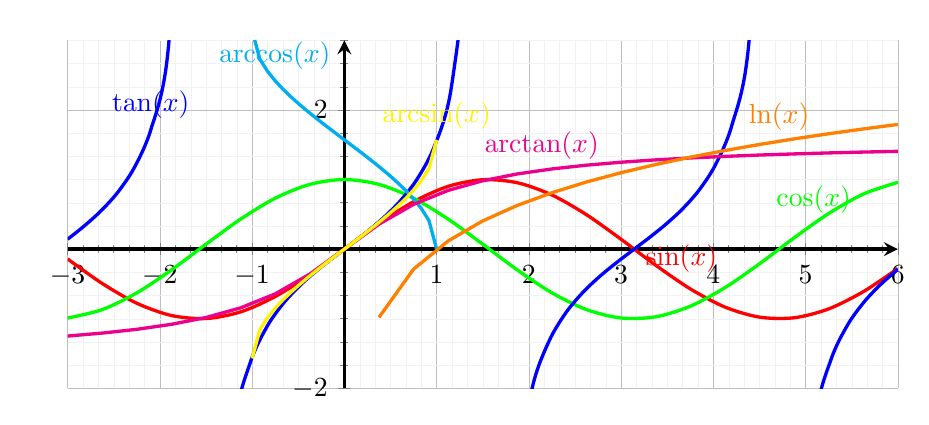
\begin{tikzpicture}
        \begin{axis}[
            axis lines = middle,
            domain = -3:6,
            ymin = -2,
            ymax = 3,
            width = \linewidth,
            height = 6cm,
            style = very thick,
            grid = both,
            grid style = {line width=.1pt, draw=gray!10},
            major grid style = {line width=.2pt,draw=gray!50},
            minor tick num = 5,
            restrict y to domain=-10:10,
        ]
        
        \addplot[red, smooth]{sin(deg(x))} node[pos=0.75] (endofplotsquare1) {};
        \node [above,color=red] at (endofplotsquare1) {$\sin(x)$};

        \addplot[green, smooth]{cos(deg(x))} node[pos=0.9] (endofplotsquare2) {};
        \node [above,color=green] at (endofplotsquare2) {$\cos(x)$};

        \addplot[blue, smooth, samples=51]{tan(deg(x))} node[pos=0.05] (endofplotsquare3) {};
        \node [above,color=blue] at (endofplotsquare3) {$\tan(x)$};
        
        \addplot[cyan, domain=-1:1]{acos(x)/180*pi} node[pos=0.2] (endofplotsquare4) {};
        \node [above,color=cyan] at (endofplotsquare4) {$\arccos(x)$};

        \addplot[magenta] {atan(x)/180*pi} node[pos=0.6] (endofplotsquare5) {};
        \node [above,color=magenta] at (endofplotsquare5) {$\arctan(x)$};

        \addplot[yellow, domain=-1:1]{asin(x)/180*pi} node[pos=1] (endofplotsquare6) {};
        \node [above,color=yellow] at (endofplotsquare6) {$\arcsin(x)$};

        \addplot[orange]{ln(x)} node[pos=0.8] (endofplotsquare7) {};
        \node [above,color=orange] at (endofplotsquare7) {$\ln(x)$};

        \end{axis}
    \end{tikzpicture}
\end{center}

\subsection*{More Integrals}
\begin{tabularx}{\linewidth}{XX}
    $\int_1^\infty \frac{1}{x^3} \sqrt{\frac{x}{x + 1}}\,dx$ & $2 \left[-\frac{1}{3}t^{-3} + t^-1\right]_{1/\sqrt{2}}^{\sqrt{\frac{a}{1 + a}}}$
\end{tabularx}

\end{document}
